\documentclass[a4paper, 12pt]{article}\usepackage[]{graphicx}\usepackage[]{color}
%% maxwidth is the original width if it is less than linewidth
%% otherwise use linewidth (to make sure the graphics do not exceed the margin)
\makeatletter
\def\maxwidth{ %
  \ifdim\Gin@nat@width>\linewidth
    \linewidth
  \else
    \Gin@nat@width
  \fi
}
\makeatother

\definecolor{fgcolor}{rgb}{0.345, 0.345, 0.345}
\newcommand{\hlnum}[1]{\textcolor[rgb]{0.686,0.059,0.569}{#1}}%
\newcommand{\hlstr}[1]{\textcolor[rgb]{0.192,0.494,0.8}{#1}}%
\newcommand{\hlcom}[1]{\textcolor[rgb]{0.678,0.584,0.686}{\textit{#1}}}%
\newcommand{\hlopt}[1]{\textcolor[rgb]{0,0,0}{#1}}%
\newcommand{\hlstd}[1]{\textcolor[rgb]{0.345,0.345,0.345}{#1}}%
\newcommand{\hlkwa}[1]{\textcolor[rgb]{0.161,0.373,0.58}{\textbf{#1}}}%
\newcommand{\hlkwb}[1]{\textcolor[rgb]{0.69,0.353,0.396}{#1}}%
\newcommand{\hlkwc}[1]{\textcolor[rgb]{0.333,0.667,0.333}{#1}}%
\newcommand{\hlkwd}[1]{\textcolor[rgb]{0.737,0.353,0.396}{\textbf{#1}}}%
\let\hlipl\hlkwb

\usepackage{framed}
\makeatletter
\newenvironment{kframe}{%
 \def\at@end@of@kframe{}%
 \ifinner\ifhmode%
  \def\at@end@of@kframe{\end{minipage}}%
  \begin{minipage}{\columnwidth}%
 \fi\fi%
 \def\FrameCommand##1{\hskip\@totalleftmargin \hskip-\fboxsep
 \colorbox{shadecolor}{##1}\hskip-\fboxsep
     % There is no \\@totalrightmargin, so:
     \hskip-\linewidth \hskip-\@totalleftmargin \hskip\columnwidth}%
 \MakeFramed {\advance\hsize-\width
   \@totalleftmargin\z@ \linewidth\hsize
   \@setminipage}}%
 {\par\unskip\endMakeFramed%
 \at@end@of@kframe}
\makeatother

\definecolor{shadecolor}{rgb}{.97, .97, .97}
\definecolor{messagecolor}{rgb}{0, 0, 0}
\definecolor{warningcolor}{rgb}{1, 0, 1}
\definecolor{errorcolor}{rgb}{1, 0, 0}
\newenvironment{knitrout}{}{} % an empty environment to be redefined in TeX

\usepackage{alltt}
\usepackage[utf8]{inputenc}
\usepackage[brazilian, english]{babel}
\usepackage{indentfirst}
\usepackage{graphicx}
\usepackage{float}
\usepackage{titlesec}
\usepackage{amsmath}
\usepackage{caption}
\usepackage{subfigure}
\usepackage{hyperref}
\usepackage{fixltx2e} %Para subscripts
\usepackage{pgfplots}
\usepackage{textcomp}
\usepackage{enumitem}
\usepackage{multicol}


\title{\textbf{Uso do Algoritmo K-means na Ilustração da Técnica de Clusterização:  um Estudo de Caso Utilizando R}}
\author{\textit{Eric Calasans de Barros}\\\textit{Fagner Freire de Oliveira}}
\IfFileExists{upquote.sty}{\usepackage{upquote}}{}
\begin{document}
	\maketitle
	
	{%
		\selectlanguage{brazilian}
		\begin{abstract}
			Diante da grande quantidade de dados que são produzidos hoje em dia se faz necessário que se conheçam técnicas estatísticas e que se tenha habilidade na utilização de ferramentas computacionais para que, assim, se possa transformar essa massiva de dados em informação útil para ser utilizada para o bem da humanidade.  Os autores apresentam um estudo de caso de uso da técnica de clusterização conhecida como \textbf{\textit{K-means}} e da linguagem \textbf{R} para análise de um conjunto de dados referentes aos índices de criminalidade e violência no Estado do Rio de Janeiro.
		\end{abstract}
	}

	{%
		\selectlanguage{english}
		\begin{abstract}
			Facing the great amount of data made nowadays it is necessary to know statistics techniques and have expertise in handling computational tools to achieve success in change this massive quantity of data in useful information that can be use for good of humankind.  The authors present a case study of application of a clustering technique named \textit{\textbf{K-means}} and \textbf{R} language in analysis of a dataset concerning to criminal indexes and violence in Rio de Janeiro.
		\end{abstract}	
	}
	\vspace{1cm}
	\textit{\textbf{Palavras-chave}:} Clusterização, K-means, R, cluster.
	
	\selectlanguage{brazilian}
	
	\begin{multicols}{2}
		\section{Introdução}
		Mineração de dados é o método de investigação de grandes quantidades de dados com o objetivo de encontrar irregularidade, padrões e correlações para arcar a tomada de decisões e possibilitar vantagens estratégicas\cite{intro1}.\\
		
		A quantidade de dados produzido está dobrando a cada dois anos. Dados não-estruturados compõem sozinhos 90\% do nosso universo digital. Entretanto, mais informação não significa necessariamente mais conhecimento. A mineração de dados nos permite filtrar todo o ruído caótico e repetitivo, entender o que é relevante e, então, fazer bom uso dessa informação para avaliar os prováveis resultados.
		
		Os resultados obtidos com a mineração de dados podem ser usados no gerenciamento de informação, processamento de pedidos de informação, tomada de decisão, controle de processo e muitas outras aplicações. A mineração de dados pode ser aplicada de duas formas: como um processo de verificação e como um processo de descoberta . No processo de verificação, o usuário sugere uma hipótese acerca da relação entre os dados e tenta prová-la aplicando técnicas como análises estatística e multidimensional sobre um banco de dados contendo informações passadas. No processo de descoberta não é feita nenhuma suposição antecipada. Esse processo usa técnicas, tais como, árvores de decisão, algoritmos genéticos e redes neurais.\\
		
		As técnicas de mineração de dados podem ser aplicadas a tarefas como classificação, estimativa, associação, sumarização e segmentação. Essas tarefas são descritas a seguir\cite{intro2}:
		\begin{itemize}
			\item \textbf{Classificação} - Reconhece modelos que descrevem o grupo ao qual o item pertence por meio do exame dos itens já classificados e pela inferência de um conjunto de regras. Equivale  a construir um modelo de algum tipo que possa ser aplicado a dados não classificados visando categorizá-los em classes.  Empresas de operadoras de cartões de crédito e companhias telefônicas preocupam-se com a perda de clientes regulares: a classificação pode ajudar a descobrir as características de clientes que provavelmente virão abandoná-las e oferecer um modelo para ajudar os gerentes a prever quem são, de modo que se elabore antecipadamente campanhas especiais para reter esses clientes;
			
			\item \textbf{Estimativa ou Regressão} - A estimativa é utilizada para determinar  valores para alguma variável contínua desconhecida como, por exemplo, lucro, distância ou saldo na poupança. Ela lida com resultados contínuos, enquanto que a classificação lida com resultados discretos. Ela pode ser usada para executar uma tarefa de classificação, convencionando-se que diferentes intervalos de valores contínuos correspondem a diferentes classes. Como exemplos de tarefas de estimativa tem-se : estimar o número de alunos de uma escola; estimar o lucro  total de uma empresa;  prever a demanda de consumidores para um novo produto;
			
			\item \textbf{Associação} - a detecção de relações entre os registros, ocorrências ligadas a um único evento. O exemplo clássico é determinar quais produtos costumam ser colocados juntos em um carrinho de supermercado; outro exemplo seria um estudo de modelos de compra em lojas de carros pode revelar que, na compra de um carro automático, 85\% das pessoas querem ele com bancada de couro;
			
			\item \textbf{Sumarização} - a tarefa de sumarização envolve métodos para encontrar uma descrição compacta para um subconjunto de dados. Um simples exemplo desta tarefa poderia ser tabular o significado e desvios padrão para todos os itens de dados;
			
			\item \textbf{Segmentação ou Clusterização} - funciona de maneira semelhante a classificação quando ainda não foram definidos grupos. Uma técnica em que através de métodos numéricos e a partir somente das informações das variáveis de cada caso, tem por objetivo agrupar automaticamente por aprendizado não supervisionado os \textbf{n} casos da base de dados em \textbf{k} grupos, geralmente disjuntos, denominados clusters ou agrupamentos.			
		\end{itemize}
	
		Um dos métodos de clusterização é o algoritmo de \textit{\textbf{Análise de Agrupamento K-means(kmeans)}}  um dos mais conhecidos e utilizados, além de ser o que possui o maior número de variações. O algoritmo inicia com a escolha dos  k elementos que formaram as sementes iniciais. Esta escolha pode ser feita de muitas formas, entre elas:
		\begin{itemize}
			\item selecionando as k primeiras observações;
			\item selecionando k observações aleatoriamente; 
			\item escolhendo k observações de modo que seus valores sejam bastante diferentes. Por exemplo, ao se agrupar uma população em três grupos de acordo com a altura dos indivíduos, poderia se escolher um indivíduo de baixa estatura, um de estatura mediana e um alto.			
		\end{itemize}
	
		Escolhidas as sementes iniciais, é calculada a distância de cada elemento em relação às sementes, agrupando o elemento ao grupo que possuir a menor distância (mais similar) e recalculando o centróide do mesmo. O processo é repetido até que todos os elementos façam parte de um dos clusters.\\
		
		Após agrupar todos os elementos, procura-se encontrar uma partição melhor do que a gerada arbitrariamente. Para isto, calcula-se o grau de homogeneidade interna dos grupos através da \textit{\textbf{Soma de Quadrados Residual (SQRes)}}, que é a medida usada para avaliar o quão boa é uma partição.\\
		
		Após o cálculo, move-se o primeiro objeto para os demais grupos e verifica-se se existe ganho na \textit{SQRes}, ou seja, se ocorre uma diminuição no valor da SQRes. Existindo, o objeto é movido para o grupo que produzir o maior ganho, a \textit{SQRes} dos grupos é recalculada e passa-se ao objeto seguinte. Depois de um certo número de iterações ou não havendo mais mudanças, o processo é interrompido.\\
				
		
		É de conhecimento público que o Estado do Rio de Janeiro(\textbf{RJ}) tem, senão o maior, um dos maiores índices de violência do País.  A mídia, por repetidas vezes, mostra não só as cenas de violência constantes no RJ mas também aponta dados estatísticos que corroboram ou complementam a informação capturada pelas câmeras.   Para ajudar no combate à violência e como forma de otimizar os recursos que são destinados à Segurança Pública, se faz necessário levantamento de dados referentes e pertinentes a esta matéria, bem como uma análise detalhada e sistematizada dos mesmos, para que sejam transformados em informação útil e confiável.\\
		
		Neste aspecto, o estudo da Estatística e suas técnicas de análise de dados, aliado ao uso de uma ferramenta computacional que possibilite ao analista acelerar os cálculos e produzir gráficos de qualidade configuram-se nos maiores aliados para esta tarefa.\\
		
		A \textbf{linguagem R(R)} foi criada originalmente no departamento de Estatística da universidade de Auckland, Nova Zelândia, por Ross Ihaka e Robert Gentleman\cite{rwiki}.  Oferece uma grande variedade de funções estatísticas e de plotagem de gráficos, bem como oferece uma facilidade na hora de produzir códigos de qualidade e softwares interativos\cite{rcite2}.  Pode ser aplicada em várias áreas do conhecimento que requeiram manipulação de dados estatísticos:  Ciências Biológicas, Sociais, Exatas, Engenharia, etc. 
		
		\section{Metodologia}
		 Os dados para análise foram obtidos diretamente do site do Instituto de Segurança Pública do Estado do Rio de Janeiro(\url{http://www.ispdados.rj.gov.br/Arquivos/BaseDPEvolucaoMensalCisp.csv})\cite{dados}, constando de uma base de dados(\textbf{DB}) contendo 23185 linhas, dispostas em 61 colunas.  De acordo com o site, as Áreas Integradas de Segurança Pública(\textbf{AISP}) foram criadas através da \textbf{Resolução SSP N. 263 de 27 de julho de 1999}, como parte de uma política de segurança pública que tinha por objetivo estreitar a ligação entre as Polícias Civil e Militar, bem como destas com as comunidades abrangidas pelas AISP através da gestão participativa na identificação e resolução dos problemas locais de segurança pública\cite{aisp}.  A figura abaixo mostra a área de jurisdição de cada AISP no RJ:
	\end{multicols}
			 %Colocar figura da AISP
	\begin{figure}[H]
		\centering
		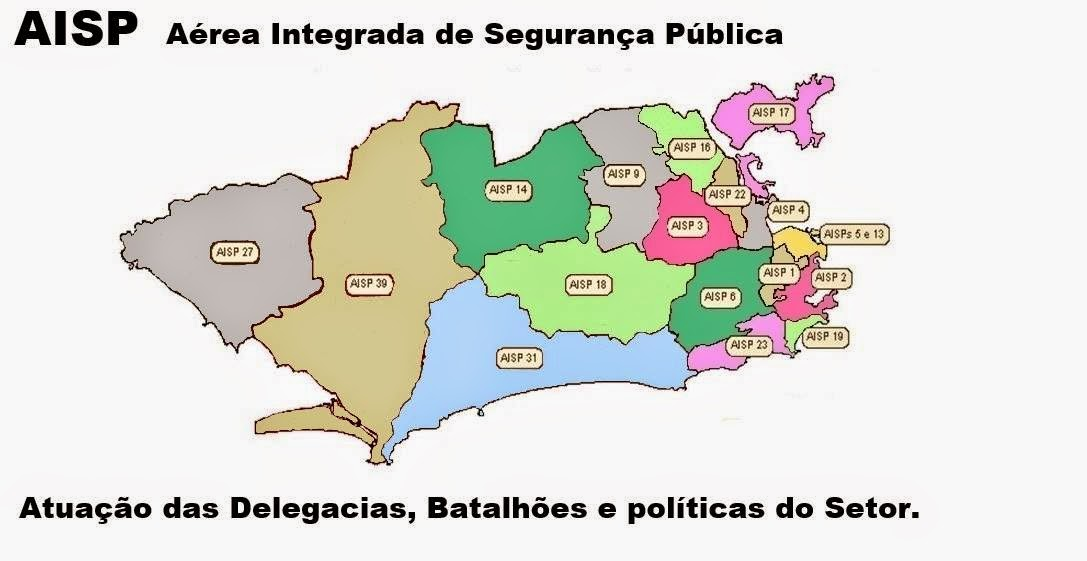
\includegraphics[width=0.8\linewidth]{aisp}
		\caption{Distribuição das AISPs}
		\label{fig:aisps}
	\end{figure}

	\begin{multicols}{2}
		  Para efeitos de estudo foram selecionadas da DB as seguintes variáveis, cuja descrição segue abaixo:
		 	\begin{itemize}
		 		\item \textbf{aisp} - Número da Área Integrada de Segurança Pública;
		 		\item \textbf{mes\_ano} - Mês e ano da comunicação da ocorrência;
		 		\item \textbf{estupro} - Estupro;
		 		\item \textbf{hom\_culposo} - Homicídio culposo(trânsito);
		 		\item \textbf{roubo\_veiculo} - Roubo de veículo;
		 		\item \textbf{hom\_doloso} - Homicídio doloso;
		 		\item \textbf{tentat\_hom} - Tentativa de homicídio;
		 		\item \textbf{estelionato} - Estelionato;
		 		\item \textbf{roubo\_celular} - Roubo de celular;
		 		\item \textbf{pessoas\_desaparecidas} - Pessoas desaparecidas.
		 	\end{itemize}
	 	A seguir os dados foram agrupados em dois subconjuntos de dados:  por \textbf{mes\_ano} e por \textbf{AISP};  desta forma a visualização da técnica de clusterização ficou mais fácil de ser percebida. \\
	 	\end{multicols}
\begin{knitrout}\footnotesize
\definecolor{shadecolor}{rgb}{0.969, 0.969, 0.969}\color{fgcolor}\begin{kframe}
\begin{alltt}
\hlkwd{library}\hlstd{(dplyr)}
\end{alltt}


{\ttfamily\noindent\color{warningcolor}{\#\# Warning: package 'dplyr' was built under R version 3.4.2}}

{\ttfamily\noindent\itshape\color{messagecolor}{\#\# \\\#\# Attaching package: 'dplyr'}}

{\ttfamily\noindent\itshape\color{messagecolor}{\#\# The following objects are masked from 'package:stats':\\\#\# \\\#\#\ \ \ \  filter, lag}}

{\ttfamily\noindent\itshape\color{messagecolor}{\#\# The following objects are masked from 'package:base':\\\#\# \\\#\#\ \ \ \  intersect, setdiff, setequal, union}}\begin{alltt}
\hlcom{#Leitura do arquivo da base de dados}
\hlstd{base} \hlkwb{<-} \hlkwd{read.csv}\hlstd{(}\hlstr{"BaseDPEvolucaoMensalCisp.csv"}\hlstd{,} \hlkwc{sep} \hlstd{=} \hlstr{';'}\hlstd{)}

\hlcom{#Agrupamento por mês}
\hlstd{porMes} \hlkwb{<-} \hlkwd{group_by}\hlstd{(base, mes_ano)} \hlopt
\hlkwd{summarise}\hlstd{(}\hlkwc{estupro}\hlstd{=}\hlkwd{sum}\hlstd{(estupro),}
\hlkwc{celular}\hlstd{=}\hlkwd{sum}\hlstd{(roubo_celular),} \hlkwc{tentHomicidio}\hlstd{=}\hlkwd{sum}\hlstd{(tentat_hom),}
\hlkwc{homDoloso}\hlstd{=}\hlkwd{sum}\hlstd{(hom_doloso),} \hlkwc{homCulposo} \hlstd{=} \hlkwd{sum}\hlstd{(hom_culposo),}
\hlkwc{rouboVeiculo}\hlstd{=}\hlkwd{sum}\hlstd{(roubo_veiculo),} \hlkwc{estelionato}\hlstd{=}\hlkwd{sum}\hlstd{(estelionato),}
\hlkwc{pessDesap}\hlstd{=}\hlkwd{sum}\hlstd{(pessoas_desaparecidas))}

\hlcom{#Agrupamento por AISP}
\hlstd{porAISP} \hlkwb{<-} \hlkwd{group_by}\hlstd{(base, AISP)} \hlopt
\hlkwd{summarise}\hlstd{(}\hlkwc{estupro}\hlstd{=}\hlkwd{sum}\hlstd{(estupro),} \hlkwc{celular}\hlstd{=}\hlkwd{sum}\hlstd{(roubo_celular),}
\hlkwc{tentHomicidio}\hlstd{=}\hlkwd{sum}\hlstd{(tentat_hom),}\hlkwc{homDoloso}\hlstd{=}\hlkwd{sum}\hlstd{(hom_doloso),}
\hlkwc{homCulposo} \hlstd{=} \hlkwd{sum}\hlstd{(hom_culposo),} \hlkwc{rouboVeiculo}\hlstd{=}\hlkwd{sum}\hlstd{(roubo_veiculo),}
\hlkwc{estelionato}\hlstd{=}\hlkwd{sum}\hlstd{(estelionato),} \hlkwc{pessDesap}\hlstd{=}\hlkwd{sum}\hlstd{(pessoas_desaparecidas))}
\end{alltt}
\end{kframe}
\end{knitrout}

		\begin{multicols}{2}
		Utilizando o R pode-se sumarizar os dados nas suas medidas estatísticas(média, máximo, mínimo, desvio-padrão) e se ter uma ideia da estatística descritiva destes conjuntos de dados:
		\end{multicols}
\begin{knitrout}\footnotesize
\definecolor{shadecolor}{rgb}{0.969, 0.969, 0.969}\color{fgcolor}\begin{kframe}
\begin{alltt}
\hlcom{#Principais variáveis estatísticas}
\hlkwd{summary}\hlstd{(porMes)}
\end{alltt}
\begin{verbatim}
##     mes_ano       estupro         celular       tentHomicidio  
##  2003m1 :  1   Min.   :188.0   Min.   : 301.0   Min.   :243.0  
##  2003m10:  1   1st Qu.:276.2   1st Qu.: 529.2   1st Qu.:325.2  
##  2003m11:  1   Median :359.0   Median : 656.5   Median :365.0  
##  2003m12:  1   Mean   :359.0   Mean   : 781.6   Mean   :388.6  
##  2003m2 :  1   3rd Qu.:428.8   3rd Qu.: 913.0   3rd Qu.:443.2  
##  2003m3 :  1   Max.   :561.0   Max.   :2548.0   Max.   :645.0  
##  (Other):168                                                   
##    homDoloso       homCulposo     rouboVeiculo   estelionato  
##  Min.   :272.0   Min.   :111.0   Min.   :1413   Min.   : 717  
##  1st Qu.:377.2   1st Qu.:175.0   1st Qu.:2052   1st Qu.:1561  
##  Median :446.0   Median :195.0   Median :2506   Median :2036  
##  Mean   :450.7   Mean   :199.1   Mean   :2524   Mean   :2121  
##  3rd Qu.:521.8   3rd Qu.:225.8   3rd Qu.:2858   3rd Qu.:2803  
##  Max.   :682.0   Max.   :299.0   Max.   :5002   Max.   :3484  
##                                                               
##    pessDesap    
##  Min.   :236.0  
##  1st Qu.:390.5  
##  Median :436.5  
##  Mean   :441.3  
##  3rd Qu.:493.8  
##  Max.   :628.0  
## 
\end{verbatim}
\begin{alltt}
\hlkwd{summary}\hlstd{(porAISP)}
\end{alltt}
\begin{verbatim}
##       AISP       estupro        celular      tentHomicidio    homDoloso   
##  Min.   : 1   Min.   : 148   Min.   :   52   Min.   : 178   Min.   : 108  
##  1st Qu.:11   1st Qu.: 697   1st Qu.:  804   1st Qu.: 824   1st Qu.: 524  
##  Median :21   Median :1268   Median : 1926   Median :1381   Median :1477  
##  Mean   :21   Mean   :1524   Mean   : 3317   Mean   :1649   Mean   :1913  
##  3rd Qu.:31   3rd Qu.:2252   3rd Qu.: 4471   3rd Qu.:2387   3rd Qu.:2651  
##  Max.   :41   Max.   :5864   Max.   :13374   Max.   :4419   Max.   :8499  
##    homCulposo      rouboVeiculo    estelionato      pessDesap   
##  Min.   :  58.0   Min.   :  104   Min.   : 1310   Min.   : 282  
##  1st Qu.: 433.0   1st Qu.:  852   1st Qu.: 4685   1st Qu.: 881  
##  Median : 668.0   Median : 4796   Median : 6919   Median :1378  
##  Mean   : 844.8   Mean   :10711   Mean   : 9003   Mean   :1873  
##  3rd Qu.:1126.0   3rd Qu.:14485   3rd Qu.:13119   3rd Qu.:2596  
##  Max.   :2498.0   Max.   :57974   Max.   :27322   Max.   :6644
\end{verbatim}
\end{kframe}
\end{knitrout}
		\begin{multicols}{2}
		Na sequência foi utilizada uma função intrínseca do R chamada \textit{\textbf{kmeans}}, que recebe como parâmetros um conjunto de dados e um número específico de centróides(maior que 2) e retorna um conjunto de dados formado por subconjuntos específicos, dos quais os de interesse para o estudo são:
			\begin{itemize}
				\item \texttt{clusters} - número do cluster associado ao dado analisado;
				\item \texttt{centers} - coordenadas dos centros passados como parâmetros após a execução da função.
			\end{itemize}
		\end{multicols}
\begin{knitrout}\footnotesize
\definecolor{shadecolor}{rgb}{0.969, 0.969, 0.969}\color{fgcolor}\begin{kframe}
\begin{alltt}
\hlcom{#Aplicação do kmeans}
\hlstd{kCelularEstuproMes} \hlkwb{<-} \hlkwd{kmeans}\hlstd{(}\hlkwd{data.frame}\hlstd{(porMes}\hlopt{$}\hlstd{celular, porMes}\hlopt{$}\hlstd{estupro),}
                             \hlkwc{centers} \hlstd{=} \hlnum{3}\hlstd{)}
\hlstd{kCelularEstuproAISP} \hlkwb{<-} \hlkwd{kmeans}\hlstd{(}\hlkwd{data.frame}\hlstd{(porAISP}\hlopt{$}\hlstd{celular, porAISP}\hlopt{$}\hlstd{estupro),}
                              \hlkwc{centers} \hlstd{=} \hlnum{3}\hlstd{)}

\hlstd{kEstuproTentHomicidioMes} \hlkwb{<-} \hlkwd{kmeans}\hlstd{(}\hlkwd{data.frame}\hlstd{(porMes}\hlopt{$}\hlstd{estupro,}
      \hlstd{porMes}\hlopt{$}\hlstd{tentHomicidio),} \hlkwc{centers} \hlstd{=} \hlnum{3}\hlstd{)}
\hlstd{kEstuproTentHomicidioAISP} \hlkwb{<-} \hlkwd{kmeans}\hlstd{(}\hlkwd{data.frame}\hlstd{(porAISP}\hlopt{$}\hlstd{estupro,}
              \hlstd{porAISP}\hlopt{$}\hlstd{tentHomicidio),} \hlkwc{centers} \hlstd{=} \hlnum{3}\hlstd{)}

\hlstd{kRouboVeiculoTentHomicidioMes} \hlkwb{<-} \hlkwd{kmeans}\hlstd{(}\hlkwd{data.frame}\hlstd{(porMes}\hlopt{$}\hlstd{rouboVeiculo,}
      \hlstd{porMes}\hlopt{$}\hlstd{tentHomicidio),} \hlkwc{centers} \hlstd{=} \hlnum{4}\hlstd{)}
\hlstd{kRouboVeiculoTentHomicidioAISP} \hlkwb{<-} \hlkwd{kmeans}\hlstd{(}\hlkwd{data.frame}\hlstd{(porAISP}\hlopt{$}\hlstd{rouboVeiculo,}
                \hlstd{porAISP}\hlopt{$}\hlstd{tentHomicidio),} \hlkwc{centers} \hlstd{=} \hlnum{4}\hlstd{)}

\hlstd{porMes} \hlkwb{<-} \hlkwd{data.frame}\hlstd{(porMes, kCelularEstuproMes}\hlopt{$}\hlstd{cluster,}
  \hlstd{kEstuproTentHomicidioMes}\hlopt{$}\hlstd{cluster, kRouboVeiculoTentHomicidioMes}\hlopt{$}\hlstd{cluster)}
\hlstd{porAISP} \hlkwb{<-} \hlkwd{data.frame}\hlstd{(porAISP, kEstuproTentHomicidioAISP}\hlopt{$}\hlstd{cluster,}
\hlstd{kEstuproTentHomicidioAISP}\hlopt{$}\hlstd{cluster, kRouboVeiculoTentHomicidioAISP}\hlopt{$}\hlstd{cluster)}
\end{alltt}
\end{kframe}
\end{knitrout}
  \begin{multicols}{2}
		Para cada subconjunto de dados o \textit{kmeans} foi aplicado nos seguintes cruzamentos de dados:
			\begin{itemize}
				\item \textit{Roubo de celular} $\times$ \textit{Casos de estupro};
				\item \textit{Casos de estupro} $\times$ \textit{Tentativa de homicídio};
				\item \textit{Roubo de veículo} $\times$ \textit{Tentativa de homicídio}.
			\end{itemize}
		O resultado foi armazendado em variáveis que depois foram acrescentadas aos respectivos subconjuntos de dados. \\
		
		Após isso foram confeccionados os gráficos onde se pode verificar a eficácia do método em agrupar os dados conforme a distância ao centróide, denotado pelo ponto marcado pelo triângulo.\\
	\end{multicols}		
	
	\begin{figure}[H]
		\centering
		\subfigure[Por mês]{
			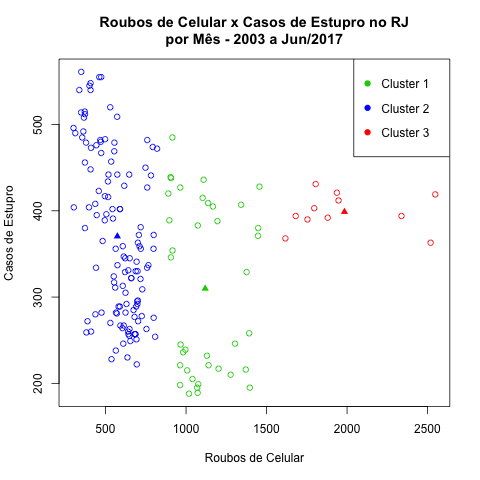
\includegraphics[width=0.4\linewidth]{celEstuproMes}}
			~
			\subfigure[Por AISP]{
				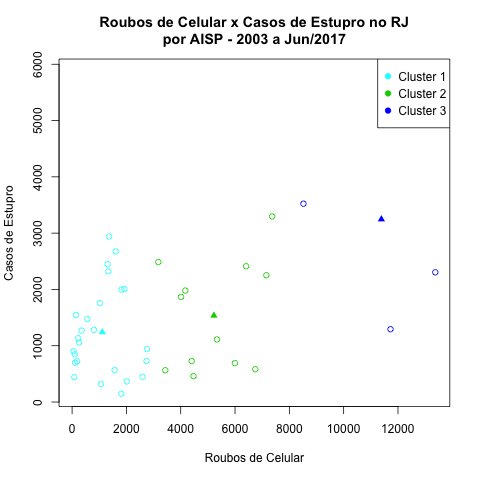
\includegraphics[width=0.4\linewidth]{celEstuproAISP}}
			\caption{Roubo de celular $\times$ Casos de estupro}
			\label{fig:celEst}
	\end{figure}
	
	\begin{figure}[H]
		\centering
		\subfigure[Por mês]{
			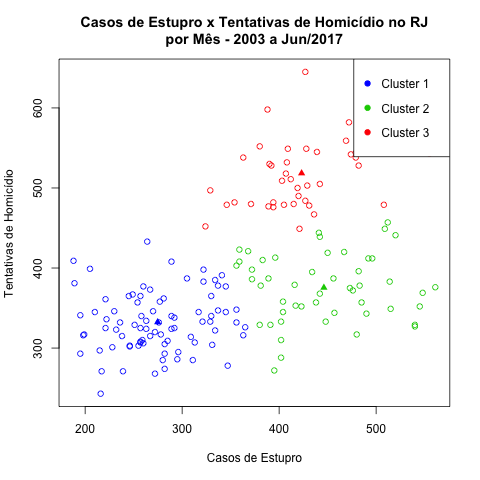
\includegraphics[width=0.4\linewidth]{estHomicidioMes}}
		~
		\subfigure[Por AISP]{
			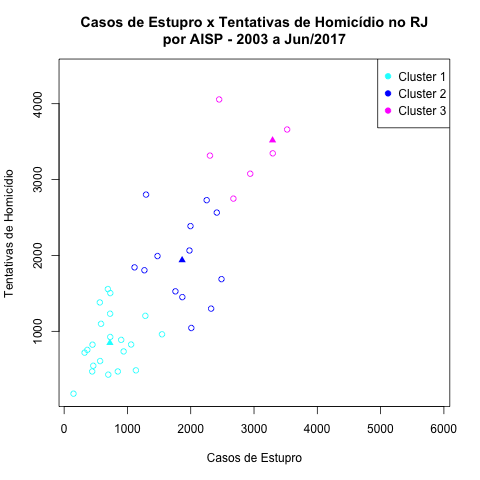
\includegraphics[width=0.4\linewidth]{estHomicidioAISP}}
		\caption{Casos de estupro $\times$ Tentativas de homicídio}
		\label{fig:estHom}
	\end{figure}

	\begin{figure}[H]
		\centering
		\subfigure[Por mês]{
			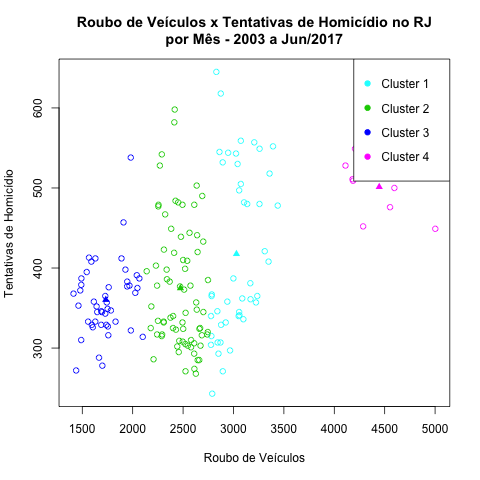
\includegraphics[width=0.4\linewidth]{rouboHomicidioMes}}
		~
		\subfigure[Por AISP]{
			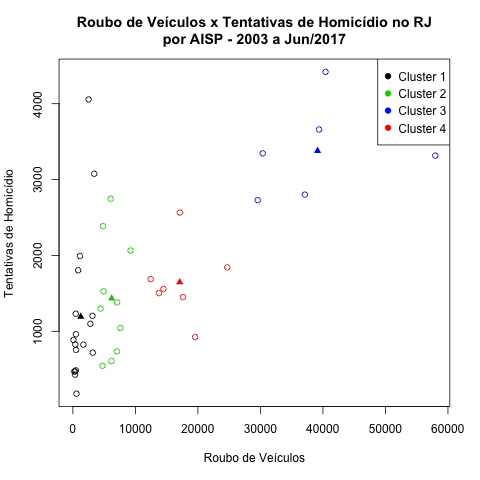
\includegraphics[width=0.4\linewidth]{rouboHomicidioAISP}}
		\caption{Roubo de veículos $\times$ Tentativas de homicídio}
		\label{fig:rouboHom}
	\end{figure}
	\begin{multicols}{2}	
		Nos gráficos relacionados ao subconjunto agrupado por mês cada ponto representa um mês no período de estudo e nos gráficos que aludem ao agrupamento por AISP os pontos representam meses no período.  
		
		\section{Conclusão}
		A técnica de clusterização \textit{kmeans} é consagrada no meio estatístico como um método eficiente para agrupar dados de acordo com um determinado critério, a saber, a distância euclidiana a um determinado centróide.  Utilizada com conhecimento, aliada a um poderoso software estatístico é capaz de extrair informação de onde aparentemente há apenas desordem e desinformação.
		
		\bibliographystyle{plain}
		\bibliography{kmeans}
		
	\end{multicols}

\end{document}
